	\newpage
\section{Podręcznik użytkownika}  %6
%Opis jak używać programu. Mogą być z zrzut ekranu razem z opisem.
\textbf{Ekran logowania}

\begin{figure}[!htb]
	\begin{center}
		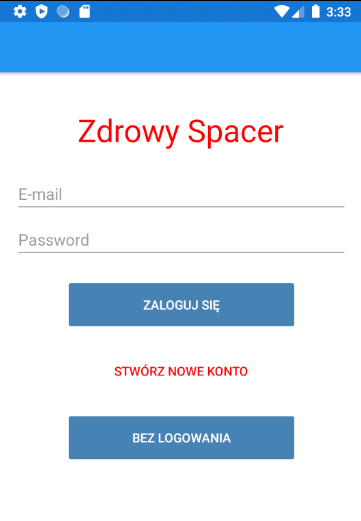
\includegraphics[width=10cm]{rys/login.png}
		\caption{Strona startowa}
		\label{rys:rysunek029}
	\end{center}
\end{figure}
 
Po włączeniu aplikacji widoczna jest strona logowania. Jeżeli użytkownik ma już utworzone konto może się zalogować poprzez wprowadzenie swojego adresu email i hasła a nastepnie naciśnięcie przycisku \textbf{zaloguj się}. Jeśli użytkownik chce utworzyć nowe konto to należy wybrać przycisk \textbf{stwórz nowe konto}. \newline

Po wybraniu opcji \textbf{stwórz nowe konto} użytkownik zostanie przeniesiony na stronę rejestracji. \newline \newline

\begin{figure}[!htb]
	\begin{center}
		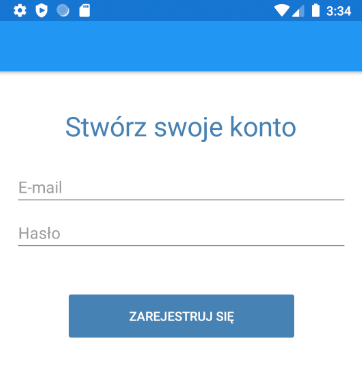
\includegraphics[width=6cm]{rys/register.png}
		\caption{Strona rejestracji}
		\label{rys:rysunek030}
	\end{center}
\end{figure}

Aby utworzyć nowe konto użytkownik musi wprowadzić prawidłowy adres email oraz hasło o długości minimum 6 znaków a następnie nacisnąć przycisk \textbf{zarejestruj się}. W przypadku poprawnego utworzenia konta użytkownik zostanie przeniesiony na stronę logowania. Jeżeli tworzenie konta się nie powiedzie pojawi się komunikat o błędzie. 

Po zalogowaniu się użytkownik zostanie przeniesiony na stronę główną.

\begin{figure}[!htb]
	\begin{center}
		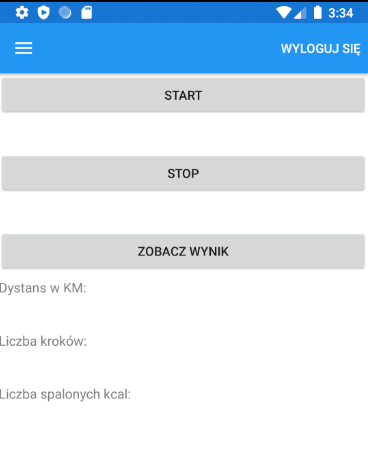
\includegraphics[width=6cm]{rys/glowna_empty.png}
		\caption{Strona główna}
		\label{rys:rysunek031}
	\end{center}
\end{figure}

Wybranie przycisku \textbf{wyloguj się} który znajduje się w prawym górnym rogu spowoduje wylogowanie z aplikacji i powrót na stronę logowania. Wybranie ikony menu, która znajduje się w prawym górnym rogu spowoduje wyświetlenie się menu bocznego.

\begin{figure}[!htb]
	\begin{center}
		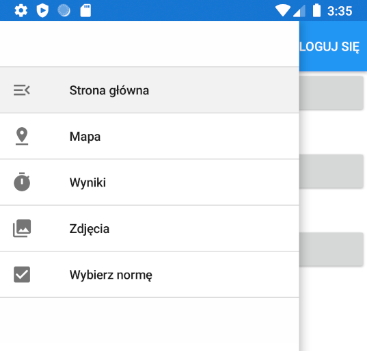
\includegraphics[width=8cm]{rys/menu.png}
		\caption{Widok po włączeniu menu bocznego}
		\label{rys:rysunek032}
	\end{center}
\end{figure}

W menu użytkownik ma do wyboru pięć opcji: strona główna, mapa, wyniki, zdjęcia, wybierz normę. W zależności od tego, którą opcję wybierze użytkownik zostanie on przekierowany na odpowiadającą swojemu wyborowi stronę.

Po wybraniu mapy użytkownik zobaczy mapę wraz ze znacznikiem określającym obecną lokalizację użytkownika.

\begin{figure}[!htb]
	\begin{center}
		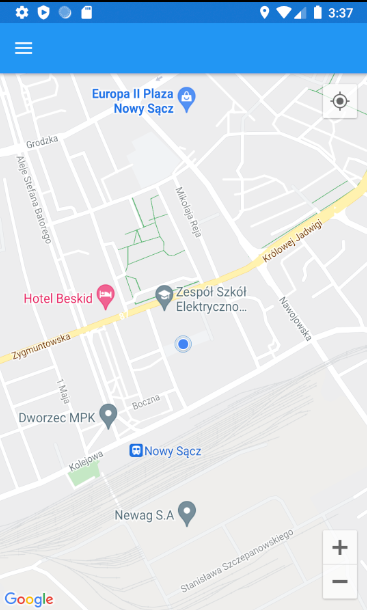
\includegraphics[width=4cm]{rys/mapa_menu.png}
		\caption{mapa}
		\label{rys:rysunek033}
	\end{center}
\end{figure}



